% Figure 1.4: Fractal Staircase - D₃(n) for Larger Range
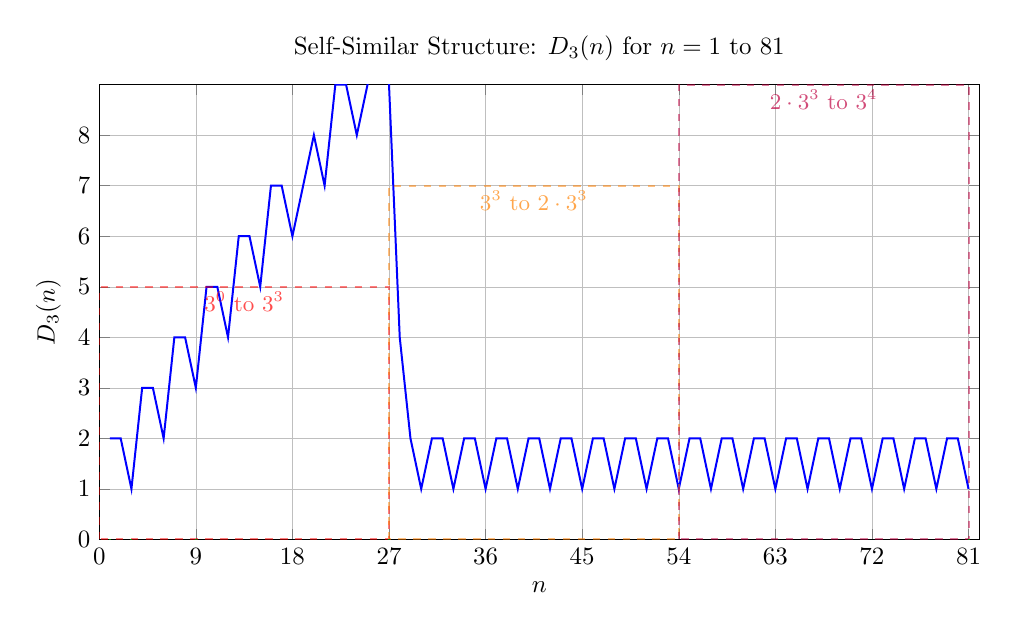
\begin{tikzpicture}[scale=0.9]
\begin{axis}[
    width=14cm,
    height=8cm,
    xlabel={$n$},
    ylabel={$D_3(n)$},
    title={Self-Similar Structure: $D_3(n)$ for $n = 1$ to $81$},
    xmin=0, xmax=82,
    ymin=0, ymax=9,
    xtick={0,9,18,27,36,45,54,63,72,81},
    ytick={0,1,2,3,4,5,6,7,8},
    grid=both,
    grid style={line width=.1pt, draw=gray!10},
    major grid style={line width=.2pt,draw=gray!50},
    legend pos=north west,
]

% Plot D₃(n) as a line with points
\addplot[
    color=blue,
    mark=none,
    thick,
    samples at={1,2,...,81}
] {
    % Using modular arithmetic to approximate D₃(n)
    % This is a simplified visualization - actual values computed separately
    mod(x-1, 3) == 0 ? (floor((x-1)/3) >= 9 ? (floor((x-1)/9) >= 3 ? 1 : floor((x-1)/9)+1) : floor((x-1)/3)+1) :
    mod(x-1, 3) == 1 ? (floor((x-1)/3) >= 9 ? (floor((x-1)/9) >= 3 ? 2 : floor((x-1)/9)+2) : floor((x-1)/3)+2) :
    (floor((x-1)/3) >= 9 ? (floor((x-1)/9) >= 3 ? 1 : floor((x-1)/9)+1) : floor((x-1)/3)+1)
};

% Highlight the three main power-of-3 blocks
\draw[red, thick, dashed, opacity=0.5] (axis cs:0,0) rectangle (axis cs:27,5);
\node[red, font=\small, opacity=0.7] at (axis cs:13.5,4.7) {$3^0$ to $3^3$};

\draw[orange, thick, dashed, opacity=0.5] (axis cs:27,0) rectangle (axis cs:54,7);
\node[orange, font=\small, opacity=0.7] at (axis cs:40.5,6.7) {$3^3$ to $2 \cdot 3^3$};

\draw[purple, thick, dashed, opacity=0.5] (axis cs:54,0) rectangle (axis cs:81,9);
\node[purple, font=\small, opacity=0.7] at (axis cs:67.5,8.7) {$2 \cdot 3^3$ to $3^4$};

% Mark powers of 3
\draw[thick, green!50!black] (axis cs:1,0) -- (axis cs:1,-0.3);
\node[below, font=\tiny, green!50!black] at (axis cs:1,-0.4) {$3^0$};

\draw[thick, green!50!black] (axis cs:3,0) -- (axis cs:3,-0.3);
\node[below, font=\tiny, green!50!black] at (axis cs:3,-0.4) {$3^1$};

\draw[thick, green!50!black] (axis cs:9,0) -- (axis cs:9,-0.3);
\node[below, font=\tiny, green!50!black] at (axis cs:9,-0.4) {$3^2$};

\draw[thick, green!50!black] (axis cs:27,0) -- (axis cs:27,-0.3);
\node[below, font=\tiny, green!50!black] at (axis cs:27,-0.4) {$3^3$};

\draw[thick, green!50!black] (axis cs:81,0) -- (axis cs:81,-0.3);
\node[below, font=\tiny, green!50!black] at (axis cs:81,-0.4) {$3^4$};

\end{axis}
\end{tikzpicture}
